%% bare_conf.tex    
%% V1.4b
%% 2015/08/26
%% by Michael Shell
%% See:
%% http://www.michaelshell.org/
%% for current contact information.
%%
%% This is a skeleton file demonstrating the use of IEEEtran.cls
%% (requires IEEEtran.cls version 1.8b or later) with an IEEE
%% conference paper.
%%
%% Support sites:
%% http://www.michaelshell.org/tex/ieeetran/
%% http://www.ctan.org/pkg/ieeetran
%% and
%% http://www.ieee.org/

\documentclass[journal]{IEEEtran} %usletter, 10 pt

\usepackage{eurosym}
\usepackage{upgreek}
\usepackage{cite}

% *** GRAPHICS RELATED PACKAGES ***
%
\ifCLASSINFOpdf
  \usepackage[pdftex]{graphicx}
  \usepackage{import}

% correct bad hyphenation here
\hyphenation{op-tical net-works semi-conduc-tor}
\usepackage[english]{babel} 
\usepackage[utf8]{inputenc}
\usepackage[]{caption}
\captionsetup{font=small}   
\usepackage{subcaption}
\usepackage{placeins}
\usepackage{color}
\usepackage{mathtools}
\usepackage{placeins}
\usepackage{relsize}
\usepackage{amssymb}
\usepackage{units}
\usepackage{amsmath}
\usepackage{float} 		
\renewcommand{\figurename}{Fig.}
\addto\captionsenglish{\renewcommand{\figurename}{Fig.}}
\usepackage{nicefrac}
\usepackage{tikz}
\usepackage[percent]{overpic}
\usepackage[hidelinks]{hyperref}

\setlength{\arrayrulewidth}{1mm}
\definecolor{mygray}{RGB}{70, 70, 70}
\definecolor{mygray2}{RGB}{40, 40, 40}
\definecolor{myred}{RGB}{255, 53, 53}
\definecolor{myblue}{RGB}{0, 70, 254}
\definecolor{myyellow}{RGB}{247, 219, 0}

\usepackage{tikz}
\usepackage[color=black,opacity=1,angle=0,scale=1]{background}
\backgroundsetup{
contents={
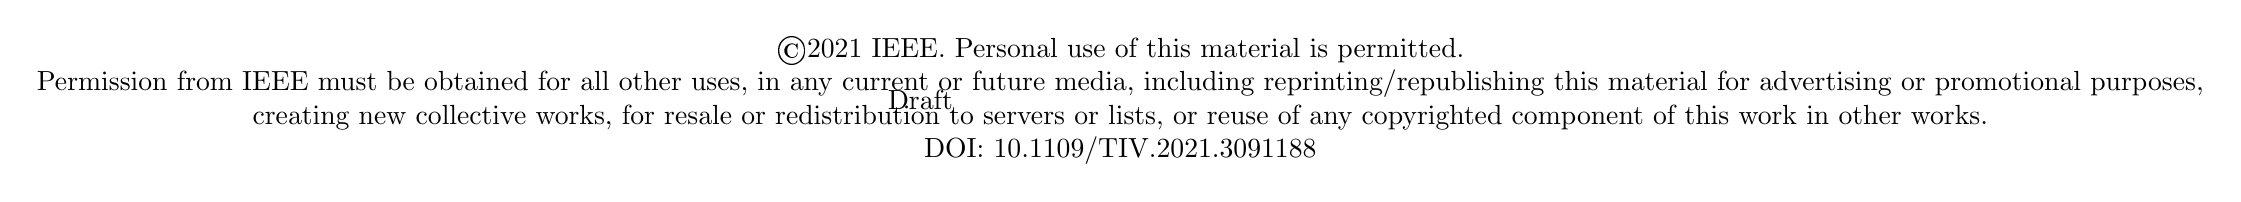
\begin{tikzpicture}
\node at (current page.center) [align=center] {\textcopyright 2021 IEEE. Personal use of this material is permitted. 
\\ Permission from IEEE must be obtained for all other uses, in any current or future media, including reprinting/republishing this material for advertising or promotional purposes, 
\\ creating new collective works, for resale or redistribution to servers or lists, or reuse of any copyrighted component of this work in other works.
\\ DOI: 10.1109/TIV.2021.3091188};
\end{tikzpicture}},
placement=bottom,
scale=0.6,
vshift=20
}

\begin{document}
\title{Online and Predictive Warning System \\\vspace{-0.0001cm} for Forced Lane Changes using Risk Maps} 
\author{Tim Puphal, Benedict Flade, Malte Probst, Volker Willert, J\"urgen Adamy and Julian Eggert \vspace{-0.25cm}
\thanks{T. Puphal, B. Flade, M. Probst and J. Eggert are with the Honda Research Institute (HRI) Europe, Carl-Legien-Str. 30, 63073 Offenbach, Germany. Email: tim.puphal@honda-ri.de 

V. Willert is with the Faculty of Electrical Engineering (FHWS), Konrad-Geiger-Str. 2, 97421 Schweinfurt, Germany. 

J. Adamy is with the Control Methods and Robotics Lab (TU Darmstadt), Landgraf-Georg Str. 4, 64283 Darmstadt, Germany.
}} 
\maketitle


\begin{abstract} 
The survival analysis of driving trajectories allows for holistic evaluations of car-related risks caused by collisions or curvy roads. This analysis has advantages over common Time-To-X indicators, such as its predictive and probabilistic nature. However, so far, the theoretical risks have not been demonstrated in real-world environments. In this paper, we therefore present Risk Maps (RM) for online warning support in situations with forced lane changes, due to the end of roads.

For this purpose, we first unify sensor data in a Relational Local Dynamic Map (R-LDM). RM is afterwards able to be run in real-time and efficiently probes a range of situations in order to determine risk-minimizing behaviors. Hereby, we focus on the improvement of uncertainty-awareness and transparency of the system. Risk, utility and comfort costs are included in a single formula and are intuitively visualized to the driver. 

In the conducted experiments, a low-cost sensor setup with a GNSS receiver for localization and multiple cameras for object detection are leveraged. The final system is successfully applied on two-lane roads and recommends lane change advices, which are separated in gap and no-gap indications. These results are promising and present an important step towards interpretable safety. 
\end{abstract}

% For peerreview papers, this IEEEtran command inserts a page break and
% creates the second title. It will be ignored for other modes.
\IEEEpeerreviewmaketitle

\begin{IEEEkeywords}
Advanced driver support system, survival analysis, risk visualization, local dynamic map, motion planning, real vehicle demonstration, risk maps.
\end{IEEEkeywords}

\section{Introduction}

The increasing complexity of source code poses a key challenge to the reliability of large-scale software systems. Software bugs in these systems can lead to safety issues~\cite{bug_safety} for users around the world as well as cause non-negligible financial losses~\cite{bug_loss}. As such, developers have to spend a large amount of time and effort on bug fixing. Consequently, \aprfull (\apr), designed to automatically generate patches to fix software bugs, has attracted wide attention from both academia and industry~\cite{long2016prophet, legoues2012genprog, long2015spr, lou2020can, tufano2018empstudy}. 


To achieve \apr, one popular approach is known as Generate-and-Validate (G\&V)~\cite{qi2015gv, ghanbari2019prapr, lou2020can, le2016hdrepair, legoues2012genprog, wen2018capgen, hua2018sketchfix, martinez2016astor, koyuncu2020fixminder, liu2019tbar, liu2019avatar}, which is typically based on the following pipeline: First, fault localization techniques~\cite{wong2016fl, abreu2007ochiai, zhang2013injecting, papadakis2015metallaxis, li2019deepfl, li2017transforming} are applied to determine the suspicious locations in programs where bugs are likely to exist. Then, the buggy locations are used by the \apr tools to generate a list of patches that replace buggy lines with correct lines. Afterward, each patch is validated against the original test suite to identify any \emph{plausible patches} (i.e., passing all tests in the test suite). Finally, to determine the \emph{correct patches}, developers examine the list of plausible patches to see if any of them can correctly fix the bug. 

Traditional \apr tools can mainly be categorized into heuristic-based~\cite{legoues2012genprog, le2016hdrepair, wen2018capgen}, constraint-based~\cite{mechtaev2016angelix, le2017s3, demacro2014nopol, long2015spr} and \template~\cite{ghanbari2019prapr, hua2018sketchfix, martinez2016astor, liu2019tbar, liu2019avatar}. Among these traditional tools, \template \apr tools~\cite{ghanbari2019prapr, liu2019tbar, benton2020effectiveness} have been able to achieve state-of-the-art results. \Template \apr tools typically leverage pre-defined templates (e.g., adding a nullness check) for bug fixing. However, since these fix templates are typically handcrafted, the number and types of bugs they are able to fix can be limited. 



To address the limitations of traditional \apr, researchers have proposed various \learning \apr tools~\cite{li2020dlfix, chen2018sequencer, jiang2021cure, lutellier2020coconut, zhu2021recoder, ye2022rewardrepair} based on the \nmtfull (\nmt) architecture~\cite{sutskever2014mt} where the input is the buggy code snippets and the goal is to translate the buggy code snippets into a fixed version. To accomplish this, \learning \apr tools require supervised training datasets with pairs of both buggy and fixed code snippets in order to learn how to perform this translation step. These training data are usually obtained by mining historical bug fixes using heuristics/keywords~\cite{dallmeier2007benchmark}, which can be imprecise for identifying bug-fixing commits; even the actual bug-fixing commits can include irrelevant code changes, leading to further pollution in the dataset~\cite{xia2022alpharepair}.
% 
Moreover, it can be hard for such \apr tools to generalize and fix bug types unseen during training. 



To better leverage recent advances in \plmfull{s} (\plm{s}), researchers~\cite{xia2022alpharepair, xia2023repairstudy, kolak2022patch, prenner2021codexws} have directly applied \plm{s} to generate patches without bug-fixing datasets. These \llm-based \apr tools work by either directly generating a complete code function~\cite{prenner2021codexws, xia2023repairstudy} or predict/infill the correct code snippet given its surrounding context~\cite{xia2022alpharepair, xia2023repairstudy}. By directly using \llm{s} that are pre-trained on billions of open-source code snippets, \llm-based \apr tools can achieve state-of-the-art performance on many repair datasets~\cite{xia2022alpharepair}. 


% 
%
%

Traditional \apr tools have long used the insight of the \emph{plastic surgery hypothesis}~\cite{barr2014plastic} where it states that the code ingredients to fix a bug already exist within the same project. Traditional \apr tools have manually designed pattern-~\cite{ghanbari2019prapr, saha2017elixir} or heuristic-based~\cite{jiang2018simfix, legoues2012genprog} approaches to finding and using such relevant code ingredients to generate fixes for bugs. However, the plastic surgery hypothesis has been largely ignored in \llm-based \apr. In fact, \llm provides a unique opportunity to fully automate the plastic surgery hypothesis idea via fine-tuning (learning project-specific information via model updates from the buggy project) and prompting (directly providing relevant code ingredients to the model), and make it directly applicable to different languages (since the \llm{s} are typically multi-lingual).%
Moreover, despite the intensive manual efforts involved, traditional \apr tools still cannot fully leverage project-specific information due to large search space for leveraging/composing existing code ingredients. In contrast, the project-specific information can effectively leveraged by \llm{s} due to their power in code understanding/vectorization, e.g., even partial/imprecise information may still guide \llm{s} in correct patch generation!
 To this end, we ask the question: \emph{How useful is the plastic surgery hypothesis in the era of \plm{s}}?








\mypara{Our Work.} To answer the question, we present \ourtech{\xspace} -- a \llm-based approach that automatically utilizes the plastic surgery hypothesis by systematically combining multiple fine-tuning and prompting strategies for \apr. \ourtech fine-tunes \plm{s} using two novel domain-specific training strategies: \textbf{\epfinetune} -- we fine-tune using the original buggy project by aggressively masking out a high percentage of tokens, which allows \plm to learn project-specific code tokens and programming styles; and \textbf{\rofinetune} -- which only masks out a single continuous code sequence per training sample, allowing the model to get used to the final \csapr task of predicting a single continuous code sequence. Furthermore, we directly leverage the ability for \plm{s} to understand natural language instructions and introduce a novel prompting strategy, \textbf{\idprompting}, which uses information retrieval and static analysis to obtain a list of relevant identifiers for the buggy lines. While such relevant identifiers are critical for fixing some difficult bugs, they may not be seen by the \llm during inference due to limited context window size. Through the use of prompting, we directly tell the model to use these extracted identifiers (relevant code ingredients) to generate the correct code. Finally, to perform repair, we combine all four model variants (including the base model, both fine-tuned models and the base model with prompting) for the final repair.





While our insight of leveraging the plastic surgery hypothesis for \llm-based \apr is generalizable across different types of \plm{s}, to implement \ourtech, we choose a recent \plm{\xspace}, \ctfive~\cite{wang2021codet5}, which is pre-trained on millions of open-source code snippets. \ctfive is an encoder-decoder model trained using \mspfull (\msp) objective where a percentage of tokens are masked out and each continuous masked token sequence is referred to as a masked span. Also, although we only extract relevant identifiers from the current buggy project (since this paper focuses on the plastic surgery hypothesis), our work can be easily extended to obtain other code information (such as relevant statements or functions) from other sources, such as  the massive pre-training corpora~\cite{husain2020codesearchnet} or historical bug-fixing datasets~\cite{jiang2019infer}, which can provide more coding knowledge for \llm{s}. Besides, although we mainly focus on using traditional string comparison algorithms for information retrieval in this paper, these techniques can be easily replaced by other frequency-based retrieval~\cite{robertson2009probabilistic} and neural search (or embedding-based search)~\cite{reimers2019sentence}.
  In summary, this paper makes the following contributions:


%


\begin{itemize}[noitemsep, leftmargin=*, topsep=0pt]
    \item \textbf{Dimension.} This paper is the first to revisit the important plastic surgery hypothesis in the era of \llm{s}. It opens up a new dimension for \llm-based \apr to incorporate previously neglected information from the buggy project itself to boost \apr performance. Furthermore, it demonstrates the promising future of retrieval-based prompting for modern \llm-based \apr.
    \item \textbf{Implementation.} We implement \ourtech based on the recent \ctfive model. We augment the model using two novel fine-tuning strategies: \epfinetune and \rofinetune, along with a novel prompting strategy based on information retrieval and static analysis: \idprompting. We combine the patches generated by all four models together and perform patch ranking to speed up \apr.% 
    \item \textbf{Evaluation Study.} We conduct an extensive evaluation against state-of-the-art \apr tools. On the widely studied \dfj 1.2 and 2.0 datasets~\cite{just2014dfj}, \ourtech is able to achieve the new state-of-the-art results of 89 and 44 correct bug fixes (15 and 8 more than best baseline) respectively.  Furthermore, we perform a broad ablation study to justify our design. \ourtech demonstrates for the first time that the plastic surgery hypothesis can substantially boost \llm-based \apr and advance state-of-the-art \apr, while being fully automated and general. Moreover, even partial/imprecise code ingredients may still effectively guide \llm{s} for \apr!
\end{itemize}


\begin{figure}
    \centering
    \setlength\tabcolsep{2pt}
    \begin{tabular}{cccl}
      \includegraphics[width=0.3\linewidth, clip, trim=150 0 35 0]{figures/fusion/activate_cells.jpg} &
      \includegraphics[width=0.3\linewidth, clip, trim=150 0 35 0]{figures/fusion/cluster.jpg} &
      \includegraphics[width=0.3\linewidth]{figures/fusion/vote.png} &
      \hspace{-2mm}
      \includegraphics[width=0.05\linewidth]{figures/fusion/colormap.pdf}
    \end{tabular}
    \caption{{\bf Combining multiple candidates.} 
          {\bf (a)} During inference, multiple cells of the network will be activated thanks to the proposed mask-based sampling strategy during training. 
          Each network cell will generate one box prediction. Here we visualize the cells by different colors according to the confidence of their corresponding box predictions. Note that the cells with the most confident prediction do not come from the center region here, but from some cells with the most discriminative textures.
          {\bf (b)} With multiple detection candidates from each local cell, we cluster them according to some simple distance threshold to correspond them to different instances.
          {\bf (c)} After a simple fusion of multiple candidate results, we can obtain a single robust result.}
    \label{fig:fusion}
  \end{figure}
\section{Probing inside Risk Maps}
\label{sec:riskmaps}
\vspace{0.02cm}
Using the R-LDM, we are able to fuse measured data into driving situations. 
However, assessing a multi-lane situation based on its risks thoroughly and, at the same time, in a fast manner remains challenging. The reason lies mostly in the variety of possible predictions for such situations. Additionally, there are underlying driving uncertainties, which arise from car sensors and likewise, e.g., from the driver behavior. 

In this context, planning methods must determine an optimal maneuver for the ego driver. With map data, the driving space was constrained and we differentiated between static paths on the one hand, and dynamic trajectories on the other hand. Still, a single path and trajectory that is safe and beneficial for the ego driver needs to be found. 
Therefore, so-called "probing" inside RiskMaps (RM) will be leveraged. We consider probing as the prediction of an ego driving motion and its evaluation of induced risks. By intelligently probing adequate numbers of fixed trajectories along paths in RM, motions will be efficiently planned. 

This section describes the concepts behind the planner RM. For this purpose, we will first explain the trajectory probing in Section \ref{subsec:traj} with RM and we will continue with the cost evaluation of risk and benefits in Section \ref{subsec:survival}. In the last Section \ref{subsec:lat} and Section \ref{subsec:warning}, we will finalize the description of RM with the extension of path probing, which ultimately allows to warn the driver. 

\begin{figure}[t!]
  \centering
  \vspace{0.06cm}
  \resizebox{0.97\linewidth}{!}{\import{img/}{single_ramps.pdf_tex}}
  \vspace{0.25cm}
  \caption{Trajectory probing within RM. Left: Ego trajectories are planned with different acceleration and braking strengths. Right: Evaluation of the risks, utilities and comforts for constant velocity of another car. The figure shows the risk calculation in more detail.}
  \label{fig:traj_variation}
\end{figure} 

\vspace{0.05cm}
\subsection{Trajectory Probing}
\label{subsec:traj}
Hereinafter, we analyze a car-to-car encounter with collision risks, depicted in Fig. \ref{fig:traj_variation}. For every ego trajectory variation $h$, constant velocity is assumed for the other car (i.e., $v=\text{const.}$). For the ego car, we predict and create variations for a piece-wise function composed of an acceleration/braking phase and a zero-acceleration, resp., constant speed segment. Technically, we first sample $N_t$ velocity profiles $v(s)$ on the path that start at the current velocity $v_0$ and end at the planned velocities $v^h$ in the future time $s$, equidistantly sampled inside $v\in[0, v_{\text{max}}]$. In total, we thus get

\vspace{-0.02cm}

\begin{equation}
v^{h} = \frac{h}{N_t-1} \cdot v_{\text{max}} \text{\hspace{0.02cm} with \hspace{0.025cm}} h \in 0, ..., N_t-1.
\end{equation}

\vspace{0.05cm}

To reach those end velocities $v^h$, the accelerations $a^h$ are afterwards calculated that are maximal with $a_{\text{max}}$ in case of an ego trajectory that corresponds to $v_{\text{max}}$. For the cases ending in a full stop $v^h=\unit[0]{m/\text{sec}}$ of the ego vehicle, the acceleration $a^h$ becomes minimal with $a_{\text{min}}$. Note that $a_{\text{min}}$ represents hereby a negative acceleration (i.e., braking motion). This leads to

\vspace{-0.5cm}

\begin{align}
\text{if } v^h > v_0\text{: \hspace{0.025cm}} a^{h} = a_{\text{max}} \cdot \frac{v^h-v_0}{v_{\text{max}}- v_0}, \\
\text{else if } v^h < v_0\text{: \hspace{0.025cm}}a^{h} = a_{\text{min}} \cdot \frac{v_0-v^h}{v_0}. 
\end{align}

\vspace{0.01cm}

The intervals with either an acceleration or braking phase are planned for the predicted durations of $s\in[0, s_a]$ or $s\in[0, s_b]$, respectively. We formulate the included times as

\begin{equation}
s_{a} = \frac{v_0}{a_{\text{max}}} \text{\hspace{0.015cm} and \hspace{0.01cm}} s_{b} = |\frac{v_0}{a_{\text{min}}}|. %\left\| \right\|
\end{equation}

\vspace{0.1cm}

\noindent The included time in the equations is denoted as $s$ since it is not the real time $t$ but the predicted time. We assume a constant velocity for the ego vehicle in the subsequent segment $[s_a, s_h]$ and $[s_b, s_h]$. The parameter $s_h$ defines the time horizon of the velocity profile and is set according to the task. Fig. \ref{fig:traj_variation} (on the left) depicts this longitudinal probing. 

In the presented planner, a target velocity $v^h = v_{\text{tar}}$ from the RM set is eventually selected based on the explicit tradeoffs between risks $R(t)$ and benefits, which are further divided into the ego utility $U(t)$ and ego comfort $O(t)$, see Fig. \ref{fig:traj_variation} on the right. In this process, at least $N_t\geq3$ ego trajectories have to be sampled so that RM can choose between an acceleration and a braking option.  
Altogether, RM could potentially represent a fast planner applicable to avoid accidents. 

The next section will now describe the mentioned costs to select an optimal motion. Using the survival analysis approach, we include probabilistic assumptions of Gaussian uncertainty (visualized as 2D, red ellipses) and of Poisson uncertainty (escape arrows for the ego cars). However, this section represents a summary of the approach. For more details, please refer to the original publication \cite{puphal2019}. We extend and show novel ways how to plan lane changes afterwards.

\vspace{-0.2cm}
\subsection{Survival Analysis}
\label{subsec:survival}

We cannot presume that predictions of other cars, e.g., constant velocity, will be followed in reality. The survival analysis thus models uncertainties for their predicted positions with 2D Gaussians that are growing over time. These uncertainties are influenced by sensor uncertainty (dominant in first steps) and behavior uncertainty (dominant in later steps). Finally, a collision probability is given by the overlap of the Gaussians from the ego vehicle and all other vehicles.\footnote{Note that this collision probability is, in the end, dependent on the relative velocity and distance of the vehicles.} 

Since risk is defined as the probability of this critical event multiplied with a damage outcome, we include a severity term in the final risk output. 
Besides collision risks, RM allow for the analysis of further critical events, such as upcoming sharp curves. More specifically, RM model the probability to lose control and skid off during lane changes. In these cases, we assume 1D Gaussians around the ego car and look at the lateral acceleration which is influenced by road curvatures.

\vspace{0.015cm}
\subsubsection{Risk Equations}
With the help of a Poisson process, we are able to accumulate probabilities over the future time $s$ (i.e., from collisions and a curve) with the damages into a single, scalar risk value $R(t)$ for the current time  $t$. In detail, we calculate the time difference between two critical events $\tau_{\text{crit}}^{-1}(s)$. Those critical events are then divided into collision rates $\tau_{\text{coll},j}^{-1}$ (with the index defining the considered other car $j$) and a curve rate $\tau_{\text{curv}}^{-1}$. 

Due to the included survival function $S$ in a Poisson process, risks that occur further away in the prediction are considered less in the risk $R(t)$. This so-called ``escape'' effect is modeled for the ego car. We thus describe $R(t)$ by 

\vspace{-0.2cm}

\begin{equation}
R(t) = \int_0^{\infty} (\sum_j \tau_{\text{coll},j}^{-1}D_{\text{coll},j}+\tau_{\text{curv}}^{-1}D_{\text{curv}})S \,ds.
\label{eq:risk}
\end{equation}  
For Eq. (\ref{eq:risk}), the severity is hereby formulated in a desired accuracy based on a collision model $D_{\text{coll}}$ and $D_{\text{curv}}$. 

\begin{figure}[t!]
  \centering
  
  \vspace*{-0.252cm}
  
  \resizebox{0.82\linewidth}{!}{\import{img/}{cost_evaluation.pdf_tex}}
  \vspace{0.1cm}
  \caption{Visualization of the driving risk (i.e., from collision and curve), utility and comfort costs. The trajectory costs are computed over the future time and then integrated with the survival analysis to obtain a single cost scalar. Note: The graphs should only give a qualitative notion of how the costs may look like.} 
  \label{fig:single_costs}
\end{figure} 

In the end, we can visualize a risk graph showing risk hot spots for the taken velocity profile that correspond to the other cars. Such a risk graph is plotted in Fig. \ref{fig:single_costs} on the top left. As an example, it shows risk spots for two separate cars, which become visible for trajectories when the ego car come closest to the other car, while the shape of the hot spots depends on the Gaussian uncertainties of the vehicles. At this point, it should be highlighted that the risk graph shows risks over the future time, which is different to common potential field visualizations, such as \cite{guo2019}.

\vspace{0.03cm}
\subsubsection{Utility and Comfort Prediction}

The target of RM is to mimize risks as well as to maximize benefits $B(t)$. The total

\noindent costs are calculated with $C(t) = R(t)-B(t) = R(t)-U(t)-O(t)$.
In this sense, we express benefits with high utility and comfort, both also depicted in Fig. \ref{fig:single_costs}. 

Utility $U(t)$ depends on the driven ego velocity $v_1$, which attempts to reduce the general required time to arrive at a goal. Additionally, we consider a desired velocity $v_d$ for individual preferences. 
For decreasing effects of $U(t)$ at higher times $s$, we multiply the components with the survival function $S$ and write 

\vspace{-0.25cm}

\begin{equation}
U(t) = \int_0^{\infty} (b^t |v_1| + b^d |v_1 - v_d|) S \,ds.
\label{eq: utility}
\end{equation} 

\vspace{0.02cm}

Comfort $O(t)$ takes ego acceleration $a_1$ and jerk $j_1$ into account and ensures less abrupt switches between selected behaviors. The major target is still to avoid risks. Consequently, comfort is also reduced over the survival function $S$. For $O(t)$, we gain
\vspace{-0.1cm}
\begin{equation}
O(t) = \int_0^{\infty} -(b^c |a_1| + b^j |j_1|) S \,ds.
\label{eq: comfort}
\end{equation} 

With the weight parameters $b^t$, $b^d$, $b^c$ and $b^j$, in both $U(t)$ and $O(t)$, the importance of risk versus benefit can be tuned. This enables us to select a single trajectory with minimal costs $c^h$ among all sampled trajectories $N_t$. Particularly, in Fig. \ref{fig:single_costs}, the first trajectory $v^1$, i.e., with $h=1$, was chosen because $c^1$ represents the smallest cost of all trajectories. With the cost graphs of $U(t)$ and $O(t)$, visualized also in the figure alongside risks $R(t)$, we can therefore intuitively indicate the underlying reason for any selection of the planner.

\subsection{Path Probing} 
\label{subsec:lat}

For the last module of the resulting warning system, this section outlines path planning. Building upon the ego trajectory probing and cost evaluation from RM, a novel path probing technique is proposed for RM. In this way, the forced lane change of the introduction is solvable. The driver has the support of the HMI, recommending a target motion. 

As already mentioned, in large multi-lane roads (i.e., highways), a driver has distinct spatial options with the possibility of performing a lane change. A forced lane change arises either for, e.g., following the navigation route, avoiding neighboring cars or both at the same time. In these instances, the lane change path and its start time and duration must be determined. The RM make tactical decisions, which are, e.g., lane changes for a future time (depicted in Fig. \ref{fig:path_blending}). 

\begin{figure}[t!]
  \centering
  \vspace{0.23cm}
  \resizebox{0.89\linewidth}{!}{\import{img/}{merge_path.pdf_tex}}
  \vspace{0.15cm}
  \caption{Signal outputs of RM. By also probing the costs for possible ego paths, we can plan tactical lane changes. Left: Blending of path options and their selection. Right: HMI with target velocity and lane change advice.}
  
  \vspace{0.05cm}
  
  \label{fig:path_blending}
\end{figure}

In detail, we compute a path change that serves to blend between centerlines of the ego lane and of a neighbouring lane. The blending begins at a longitudinal distance $l_{\text{start}}$, which is defined as
\vspace{-0.06cm}
\begin{equation}
l_{\text{start}} = v_0 \cdot s_{\text{start}}.
\end{equation}
Accordingly, this distance $l_{\text{start}}$ depends on the current velocity $v_0$ and the future time $s_{\text{start}}$. The length of the blending interval $l_{\text{blend}}$ is, in contrast, influenced by the current, lateral distance $d_{\text{path}}$ between the two path options. Since the segment end $l_{\text{end}}$ is composed of $l_{\text{start}}$ and $l_{\text{blend}}$, we retrieve
\vspace{0.03cm}
\begin{equation}
l_{\text{end}} =  l_{\text{start}} + l_{\text{blend}} = l_{\text{start}} + v_0\sqrt{l_c \cdot d_{\text{path}}}.  
\label{eq:path_length}
\end{equation}

\vspace{0.03cm}

\noindent In Eq. (\ref{eq:path_length}), the parameter $l_c$ defines the scale factor for the increase. Simply put, for higher $l_c$, the lane change would also take more time.

In a final, next step, we blend the ego path $\mathbf{p}_{\text{ego}}(l)$ into the neighboring path $\mathbf{p}_{\text{other}}(l)$ within the segment $l_{\text{blend}}$, using a sigmoidal weighting term $w^*(l)$. Paths from Section~\ref{subsec:map} are initially resampled with evenly spaced points. The computed lane change path $\mathbf{p}_{\text{blend}}(l)$ then follows, with 
\vspace{0.07cm}
\begin{equation}
\mathbf{p}_{\text{blend}}(l) = (1-w^*(l)) \cdot \mathbf{p}_{\text{ego}}(l) + w^*(l) \cdot \mathbf{p}_{\text{other}}(l). 
\end{equation}

\vspace{0.08cm}

\noindent Generally, linear blending is achieved via the term
\vspace{0.05cm}
\begin{equation}
w(l) = \frac{l - l_{\text{start}}}{l_{\text{blend}}}, \text{with } l\in[l_{\text{start}}, l_{\text{end}}].
\end{equation}

\vspace{0.05cm}

\noindent and we thus utilize the weight $w(l)$ in a sigmoidal weight function $w^*(l)$ to gain
\vspace{0.05cm}
\begin{equation}
\vspace*{-0.1cm}
w^*(l) = \frac{{\fontsize{6}{8}\selectfont 1}}{1+e^{\mbox{\fontsize{9}{9.5}\selectfont{$-k(w(l)+0.5$)}}}}.
\vspace*{0.19cm}
\end{equation}
The constant $k$ allows to hereby tune the blending steepness and should be set to achieve a smooth blending. 
\vspace{0.05cm}

Fig. \ref{fig:path_blending} (left box) depicts two prototypical paths. They are calculated with the aforesaid variables. Note that points in the path have to be sampled densely enough for a reasonable blending. With the path blending, we can initiate an immediate lane change by setting $s_{\text{start}}=\unit[0]{\text{sec}}$, while a tactical change is obtained with, e.g., $s_{\text{start}}\hspace{-0.02cm}=\hspace{-0.02cm}\unit[2]{\text{sec}}$. A utility offset is necessary for the costs in order to incentivize the planner making a lane change. After all, RM choose the path based on its costs. 

\subsection{Selection and Warning}
\label{subsec:warning}

For multiple paths, the path blending is done iteratively. With the total path number $M_p$, ultimately, $M_{\text{p}} \cdot N_{\text{t}}$ samples are generated in RM, since ego trajectories are varied on each path. We select a single trajectory with the lowest costs for obtaining the target velocity $v_{\text{tar}}$ as well as the target path $\mathbf{p}_{\text{tar}}$. In other words, RM probe in longitudinal and lateral directions. The runtime of RM is constant because we have a fixed sample size. This suits very well for real-time purposes. In the case of Fig. \ref{fig:path_blending}, we get $M_p=2$ and sample $2 \cdot N_{\text{t}}$ trajectories. 

The planned, safe motion is now transferred into a driver suggestion or warning in an HMI so that it is explained to the driver. 
We compare the planned with the actual one to infer a warning. 

As shown in Fig. \ref{fig:path_blending} (right-hand side), the developed HMI contains a velocity scale with the current velocity $v_0$ and the safe velocity $v_{\text{tar}}$. Depending on the difference $|v_0-v_{\text{tar}}|$, the driver needs to change its behavior (accelerate, brake, etc.). Furthermore, a directional arrow depicts the path choice from the planner, which can be either ``left'', ``straight'' or ``right''. The driver should make a lane change, i.e., left, right, or stay on the lane, i.e., straight motion. The figure shows some output examples of the HMI, which are derived from the solution of the planner.
\vspace{0.12cm}


We present in section~\ref{ssec:faces} an application of PnP-HVAE on face images, using a pretrained state-of-the-art hierarchical VAE. 
Next, we study the application of our framework to natural images. To that end, we introduce  in section~\ref{ssec:patchVDVAE}  a patch hierachical VAE architecture, that is able to model natural images of different resolutions. In section~\ref{ssec:app_nat}, we provide deblurring, super-resolution and inpainting experiments to demonstrate the relevance of the proposed method.

Additional results are presented in Appendix~\ref{app:add}. All experiments can be reproduced using the code available at \url{https://github.com/jprost76/PnP-HVAE}.



\subsection{Face Image restoration (FFHQ)}\label{ssec:faces}
We first demonstrate the effectiveness of PnP-HVAE on highly structured data, by performing face image restoration.
Latent variable generative models can accurately model structured images such as face images \cite{karras2019style,vahdat2020nvae,child2021very,kingma2018glow}, and then be used to produce high quality restoration of such data. 
In our experiments, we use the VDVAE model of~\cite{child2021very}, pre-trained on the FFHQ dataset~\cite{karras2019style}, as our hierarchical VAE prior.
VDVAE has $L=66$ latent variable groups in its hierarchy and generates images at resolution $256\times256$.

We compare PnP-HVAE with the intermediate layer optimization algorithm (ILO)~\cite{daras2021intermediate} that is based on a different class of generative models than HVAE. ILO is a GAN inversion method which optimizes the image latent code along with the intermediate layer representation of a StyleGAN to generate an image consistent with a degraded observation.
We use the official implementation of ILO, along with a StyleGAN2 model~\cite{karras2020analyzing, stylegan2pytorch}, that was trained for 550k iterations on images of resolution $256\times256$ from FFHQ.  
As VDVAE and StyleGAN models are not trained on the same train-test split of FFHQ, we chose to evaluate the methods on a subset of 100 images from the CelebA dataset~\cite{liu2018large}. 
For super-resolution, the degradation model corresponds to the application of a gaussian low-pass filter followed by a $\times 4$ sub-sampling, and the addition of a gaussian white noise with $\sigma=3$.
For the deblurring, we considered motion blur and  gaussian kernels, both with a noise level $\sigma=8$. %

We provide quantitative comparisons in table~\ref{table:comp_ILO}, along with a visual comparison of the results in figure~\ref{fig:face_restoration}.
PnP-HVAE has the best  PSNR and SSIM results for all the considered restoration tasks, while ILO provides better results  for the perceptual distance.
By jointly optimizing the image and its latent variable, PnP-HVAE provides  results that are both realistic and consistent with the degraded observation.
On the other hand,  ILO  only optimizes on an extended latent space. This method generates  sharp and realistic images with better LPIPS scores,   
but the results lack  of consistency with respect to the observation, which explains the overall lower PSNR performance. 






\subsection{PatchVDVAE: a HVAE for natural images}\label{ssec:patchVDVAE}
Available generative models in the literature operate on images of  fixed resolutions and
are either restrained to datasets of limited diversity, or even to registered face images~\cite{kingma2018glow,child2021very, vahdat2020nvae, karras2019style}, or requiring additional class information~\cite{brock2018large, dhariwal2021diffusion, song2020score, luhman2022optimizing}.
Fitting an unconditional model on natural images appears to be a more difficult task, as their resolution can change, and their content is highly diverse.
The complexity of the problem can be reduced by learning a prior model on patches of reduced dimension. 
For image restoration problems, the patch model can be reused on images of higher dimensions~\cite{zoran2011learning,prost2021learning,altekruger2022patchnr}. When the model is a full CNN, the prior on the set of the  patches can  be computed efficiently by applying the network on the full image~\cite{prost2021learning}.

We thus introduce  patchVDVAE, a fully convolutional hierarchical VAE.
Contrary to existing HVAE models whose resolution is constrained by the constant tensor at the input of the top-down block, patchVDVAE can generate images of different resolutions by controlling the dimension of the input latent. 
This amounts to defining a prior on patches whose dimension corresponds to the receptive field of the VAE. A similar model is used for image denoising in~\cite{prakash2021interpretable}.

 
For PatchVDVAE architecture, we use the same bottom-up and top-down blocks as VDVAE~\cite{child2021very}, and replace the constant trainable input in the first top-down block by a latent variable, to make the model fully convolutional (details on the  architecture are given in Appendix~\ref{app:details}). 
The training dataset is composed of $128\times 128$ patches extracted from a combination of DIV2K~\cite{agustsson2017ntire} and Flickr2K~\cite{Lim_2017_CVPR_workshops} datasets.
We perform data augmentation by extracting  patches at $3$ resolutions: HR-images and $\times 2$ and $\times 4$ downscaled images. 
The model is trained for $7.10^5$ iterations with a batch size of $64$. Following the recommendation of~\cite{hazami2022efficient}, we use Adamax optimizer with an exponential moving average and gradient smoothing of the variance.
We set the decoder model to be a gaussian with diagonal covariance, as in~\cite{luhman2022optimizing}.
PatchVDVAE is fully convolutional and can generate images of dimension that are multiples of $64$ as illustrated by
figure~\ref{fig:vdvae}.

\newlength{\patchwidth}
\setlength{\patchwidth}{0.135\columnwidth}
\begin{figure}[!ht]
    \centering
    \begin{subfigure}[t]{.34\columnwidth}\hspace{0.1cm}
        \setlength{\tabcolsep}{0.02pt}
\renewcommand{\arraystretch}{0}
        \begin{tabular}{*{2}{p{1.03\patchwidth}}}
            \includegraphics[width=\patchwidth]{figures_arxiv/patchVDVAE/samples/generated/64x64/setup-5-image-0018.png} &
            \includegraphics[width=\patchwidth]{figures_arxiv/patchVDVAE/samples/generated/64x64/setup-5-image-0016.png} \\
            \includegraphics[width=\patchwidth]{figures_arxiv/patchVDVAE/samples/generated/64x64/setup-5-image-0008.png} &
            \includegraphics[width=\patchwidth]{figures_arxiv/patchVDVAE/samples/generated/64x64/setup-5-image-0019.png}   
        \end{tabular}
    \end{subfigure}\hspace{-0.15cm}
    \begin{subfigure}[t]{.64\columnwidth}
\begin{tabular}{cc}\vspace{-0.1cm}
\includegraphics[width=2\patchwidth]{figures_arxiv/patchVDVAE/samples/generated/256x256/setup-2-image-0009.png}&
        \includegraphics[width=2\patchwidth]{figures_arxiv/patchVDVAE/samples/generated/256x256/setup-2-image-0002.png}\end{tabular}

    \end{subfigure}
    \caption{\label{fig:vdvae} Left: $64\times64$ patches samples from our patchVDVAE model trained on patches from natural images.
    Right: PatchVDVAE is fully convolutional and it can generate images of higher resolution (here: $128\times128$).\vspace{-0.2cm}}
\end{figure}

\subsection{Natural images restoration}\label{ssec:app_nat}
We  evaluate PnP-HVAE on natural image restoration.
For each task, we report the average value of the PSNR, the SSIM, and the LPIPS metrics on $20$ images from the test set of the BSD dataset~\cite{MartinFTM01}.\\


\noindent
{\bf Image deblurring.}
In the experiments, we consider $2$ gaussian kernels and $2$ motion blur kernels from~\cite{levin2009understanding}, with $3$ different noise levels 
$\sigma \in \{2.55, 7.65, 12.75\}$.
As a baseline we consider  EPLL~\cite{zoran2011learning}, which learns a prior on image patches with a gaussian mixture model.
We also compare PnP-HVAE  with PnP-MMO and GS-PnP, $2$ competing convergent Plug-and-Play methods based on CNN denoisers.
PnP-MMO~\cite{pesquet2021learning} restricts the denoiser to be contraction in order to guarantee the convergence of the PnP forward-backard algorithm. GS-PnP~\cite{hurault2022gradient} considers a gradient step denoiser and reaches state-of-the-art performances of non converging methods~\cite{zhang2021plug}.
We set the temperature $\tau$  in our method as $0.95$, $0.8$ and $0.6$ for noise levels $2.55$, $7.65$ and $12.75$ respectively, and we let it run for a maximum of $50$ iterations. 
For the three compared methods we use the official implementations and pre-trained models provided by the respective authors. 
Details on the choice of hyperparameters for the concurrent methods are provided in the Appendix~\ref{app:details}
Figure~\ref{fig:deblurring_bsd} illustrates that our method provides correct deblurring results. 

According to table~\ref{tab:deb}, the performance of PnP-HVAE is between those of EPLL and GS-PnP and it outperforms PnP-MMO for large noise levels.\\

\begin{table}
\begin{center}\footnotesize
    \begin{tabular}{>{\centering}m{.3cm}*{5}{c}}
    $\sigma$ &Method & PSNR$\uparrow$ & SSIM$\uparrow$ & LPIPS$\downarrow$  \\ 
    \hline
    \multirow{4}{*}{\vcell{$2.55$}}
    & PnP-HVAE & $27.75$ & $0.79$ & $0.31$\\
    & GS-PNP \cite{hurault2022gradient} & $\mathbf{29.59}$ & $\mathbf{0.84}$ & $\mathbf{0.22}$\\
    & EPLL \cite{zoran2011learning} & $26.49$ & $0.71$ & $0.36$\\ 
    & PnP-MMO \cite{pesquet2021learning} & $\underbar{29.50}$ & $\underbar{0.83}$ & $\underbar{0.20}$ \\ \hline
    \multirow{4}{*}{\vcell{$7.65$}}
    & PnP-HVAE & $\underbar{26.36}$ & $\underbar{0.72}$ & $\underbar{0.40}$\\
    & GS-PNP \cite{hurault2022gradient} & $\mathbf{27.33}$ & $\mathbf{0.77}$ & $\mathbf{0.31}$\\
    & EPLL \cite{zoran2011learning} & $24.04$ & $0.66$ & $0.45$ \\ 
    & PnP-MMO \cite{pesquet2021learning} & $25.34$ & $0.69$ & $0.34$\\
    \hline
    \multirow{4}{*}{\vcell{$12.75$}}
    & PnP-HVAE & $\underbar{25.12}$ & $\mathbf{0.73}$ & $\underbar{0.47}$\\
    & GS-PNP \cite{hurault2022gradient} & $\mathbf{26.32}$ & $\mathbf{0.73}$ & $\mathbf{0.37}$\\
    & EPLL \cite{zoran2011learning} & $23.28$ & $0.61$ & $0.51$ \\ 
    & PnP-MMO \cite{pesquet2021learning} & $22.42$ & $0.53$& $0.54$ \\
    \hline
    &\vspace*{-.3cm}\\
            \multicolumn{2}{c}{Blur and motion kernels}& \multicolumn{3}{c}{
        \includegraphics*[scale=1]{figures_arxiv/kernels/4.png}\;\includegraphics*[scale=1]{figures_arxiv/kernels/7.png}\;\includegraphics*[scale=1]{figures_arxiv/kernels/9.png}\;\includegraphics*[scale=1]{figures_arxiv/kernels/11.png}} 
    \end{tabular}
        \caption{\label{tab:deb}Comparison  of PnP-HVAE  and other restoration methods on deblurring. Results are averaged on $4$ kernels.\vspace{-0.2cm}}% on image deblurring.}
    \end{center}
\end{table}

\begin{figure}
    
    \begin{subfigure}[h]{\linewidth}
        \centering
        \includegraphics*[width=\columnwidth]{figures_arxiv/deb_s255_k7.pdf}\vspace{-0.1cm}
        \caption{Gaussian blur, $\sigma=2.55$}
    \end{subfigure}
    \begin{subfigure}[h]{\linewidth}
        \centering
        \includegraphics*[width=\columnwidth]{figures_arxiv/deb_s765_k11.pdf}\vspace{-0.1cm}
        \caption{Motion blur, $\sigma=7.65$}
    \end{subfigure}\vspace*{-0.1cm}
    \caption{\label{fig:deblurring_bsd} Natural image deblurring\vspace{-0.1cm}}
\end{figure}

\noindent {\bf Effect of the temperature.}
PnP-HVAE gives control on the temperature of the prior over the latent space.
In figure~\ref{fig:temp_effect}, we illustrate that reducing the temperature increases the strength of the regularization prior. In this example the tuning $\tau=0.7$ produces the best performance.\\
\begin{figure}[!ht]
   
    \includegraphics[width=\columnwidth]{figures_arxiv/demo_temp.pdf}\vspace{-0.15cm}
    \caption{ \label{fig:temp_effect} Effect of the temperature in PnP-VAE on a deblurring problem, with $\sigma=7.65$.\vspace{-0.15cm}}
\end{figure}


\noindent
{\bf Image inpainting.}
Next we consider the task of noisy image inpainting. 
We compose a test-set of 10 images from the validation set of BSD~\cite{MartinFTM01} and we create masks
  by occluding diverse objects of small size in the images. 
A gaussian white noise with $\sigma=3$ is added to the images.
As a comparaison, we still consider GS-PnP and EPLL.
For PnP-HVAE, the temperature is set to $\tau=0.6$, and the algorithm is run for a maximum of $200$ iterations, unless the residual $||\x_{k+1}-\x_k||$ is on a plateau.
We provide on Table~\ref{tab:inpainting_bsd} the distortion metrics with the ground truth, as well as a visual
\begin{table}



\begin{center}
    \begin{tabular}{cccc}
        & PSNR$\uparrow$ & SSIM$\uparrow$ &LPIPS$\downarrow$ \\\hline
        PnP-HVAE  & $\mathbf{29.54}$ & $\mathbf{0.93}$ & $\mathbf{0.06}$\\
        GS-PNP & $28.52$ & $\mathbf{0.93}$ & $0.09$\\
        EPLL & $\underline{29.16}$ & $\mathbf{0.93}$ & $\mathbf{0.06}$\\
    \end{tabular}
    \caption{\label{tab:inpainting_bsd}Quantitative evaluation for inpainting on BSD.}
    \end{center}
\end{table}
comparison on figure~\ref{fig:inpainting_bsd}. 
With its hierarchical structure,  PnP-HVAE outperforms the compared methods. \vspace{0.05cm}



\begin{figure}[!h]
    \includegraphics[width=\columnwidth]{figures_arxiv/demo_inp_bsd2.pdf}\vspace{-0.1cm}
    \caption{\label{fig:inpainting_bsd}Natural image inpainting\vspace{-0.3cm}}
\end{figure}












%%%%%%%%%%%%%%%%
\section{Outlook}
\label{sec:Out}
%%%%%%%%%%%%%%%%

In this review we have attempted to present the main ideas behind the hypothesis
that the applicability of fluid dynamics to early phases of QGP dynamics can be
explained by a far-from-equilibrium hydrodynamic attractor. We have emphasised
the role of the kinematic setting specific to heavy-ion collisions, which makes
it plausible that such an attractor occurs also in QCD.  At the conceptual level
this picture is rather compelling. However, Bjorken flow is a very restrictive
setting, and despite some existing applications using the attractor in practical
calculations of phenomenologically interesting observables requires developing
effective methods of working with models with a large number of degrees of
freedom. Progress is likely to come gradually, by learning how to deal with
models of increasing complexity, extending the studies reviewed in Sections
\ref{sec:PhaseSpace} and \ref{sec:beyond}. 

The idea of hydrodynamic attractors has been closely connected with the
divergence of the hydrodynamic gradient expansion. In this review we have not
discussed this connection beyond its utilitarian aspects, but on a conceptual
level there have been some important developments in recent times. This includes
a proof of the generic divergence of the gradient expansion at the linearised
level without any symmetry assumptions, and its connection with the properties
of dispersion relations~\cite{Withers:2018srf,Heller:2020uuy}.  At the nonlinear
level, some of the results for Bjorken flow have been generalised to a much
wider class of flows, called longitudinal flows. In particular, the gradient
expansion has been shown to diverge for this class of
solutions~\cite{Heller:2021oxl}. It was also found that the large order
behaviour of the gradient series can be expressed in terms of new degrees of
freedom, the singulant fields, which track transient
effects~\cite{Heller:2021yjh}. The relevance of these advances to the study of
attractors remains an interesting challenge for the future. 

A number of issues were not addressed in this review. One is the presence of
other degrees of freedom, such as those  connected with chiral symmetry
breaking, and their possible effect on the attractor dynamics of
QGP~\cite{Mitra:2020mei,Mitra:2020hbj} (see also Ref.~\cite{Mitra:2022uhv}).
Another such issue is the role of fluctuations, which has been mostly neglected
in the attractor literature, with the notable exception of
Refs.~\cite{Akamatsu:2016llw,Chen:2022ryi}. 

It would also be very interesting to understand the role of quantum effects in
the early-time dynamics. Of course the hydrodynamic picture implicitly contains
them, but in a rather opaque way. On the other hand, the kinetic theory
description arises from quantum field theory through a series of
approximations~\cite{Mueller:2002gd,Jeon:2004dh} and it should be possible to
study the origin and robustness of the kinetic theory attractor in a framework
which allows for a systematic incorporation of quantum corrections. This is
connected with other approaches to early-time dynamics, including those
involving ideas such as the Color Glass Condensate or non-thermal
attractors~\cite{Berges:2008wm,Mazeliauskas:2018yef,Brewer:2019oha,Brewer:2022ifw,Brewer:2022vkq,Berges:2020fwq}.
It is not yet fully understood how they are related to the ideas reviewed here,
and clarifying this appears to be a very promising avenue for future research. 

Finally, there is the more general question about far-from-equilibrium
attractors in nonequilibrium systems.  In the context of heavy-ion collisions
the specific kinematic circumstances have lead us to consider boost-invariant
expansion where far-from-equilibrium hydrodynamic behaviour was first noted, but
there could be other situations where analogous phenomena might
appear~\cite{Baggioli:2021tzr}, perhaps even in the non-relativistic
domain~\cite{Le:2022ntg}.  Another context where far from equilibrium
hydrodynamic attractors can occur is the dynamics of systems in nontrivial
spacetime backgrounds (see e.g. Ref.~\cite{Vyas:2022hkm}). 




% use section* for acknowledgment
\section*{Acknowledgment}
\noindent This work has been supported by the European Union's Hori- zon 2020 project \textit{VI-DAS}, under the grant agreement number 690772. The authors would like to thank all project partners of the \textit{VI-DAS} demonstrations.

\bibliographystyle{IEEEtran}
\bibliography{bib}

% that's all folks
\end{document}


